\subsection{Hermits}

Let \(X_i = X_i(L_i)\) be the set of possible production vectors of person \(i\)
under labour constraint \(L_i\). Since we can always throw away stuff, we
assume \(X_i\) has the property\footnote{
	Careful readers might have noticed that the shape of \(X_i\) changes greatly
	depending on the space we are allowed to pick \(x\) from. The two main spaces
	of interest are \(\real_{\ge 0}^\dims\) and \(\real^\dims\). It is often more
	convenient to define \(X\) as a subset of the former. But it is not
	complicated to translate those examples to \(\real^\dims\) by applying the
	\ref{eq: lower layer} property. This will become essential in
	Section~\ref{sec: inputs and time}. Until then we will be a bit vague about
	it.
}
\[
	\label{eq: lower layer}
	\tag{lower layer}
	y\in X_i \text{ and } x\preceq y \implies x\in X_i.
\]
Where \(x \preceq y\) should be understood entry wise, i.e. \(x^{(i)} \le
y^{(j)}\) for all \(j\).

\begin{figure}
	\centering
	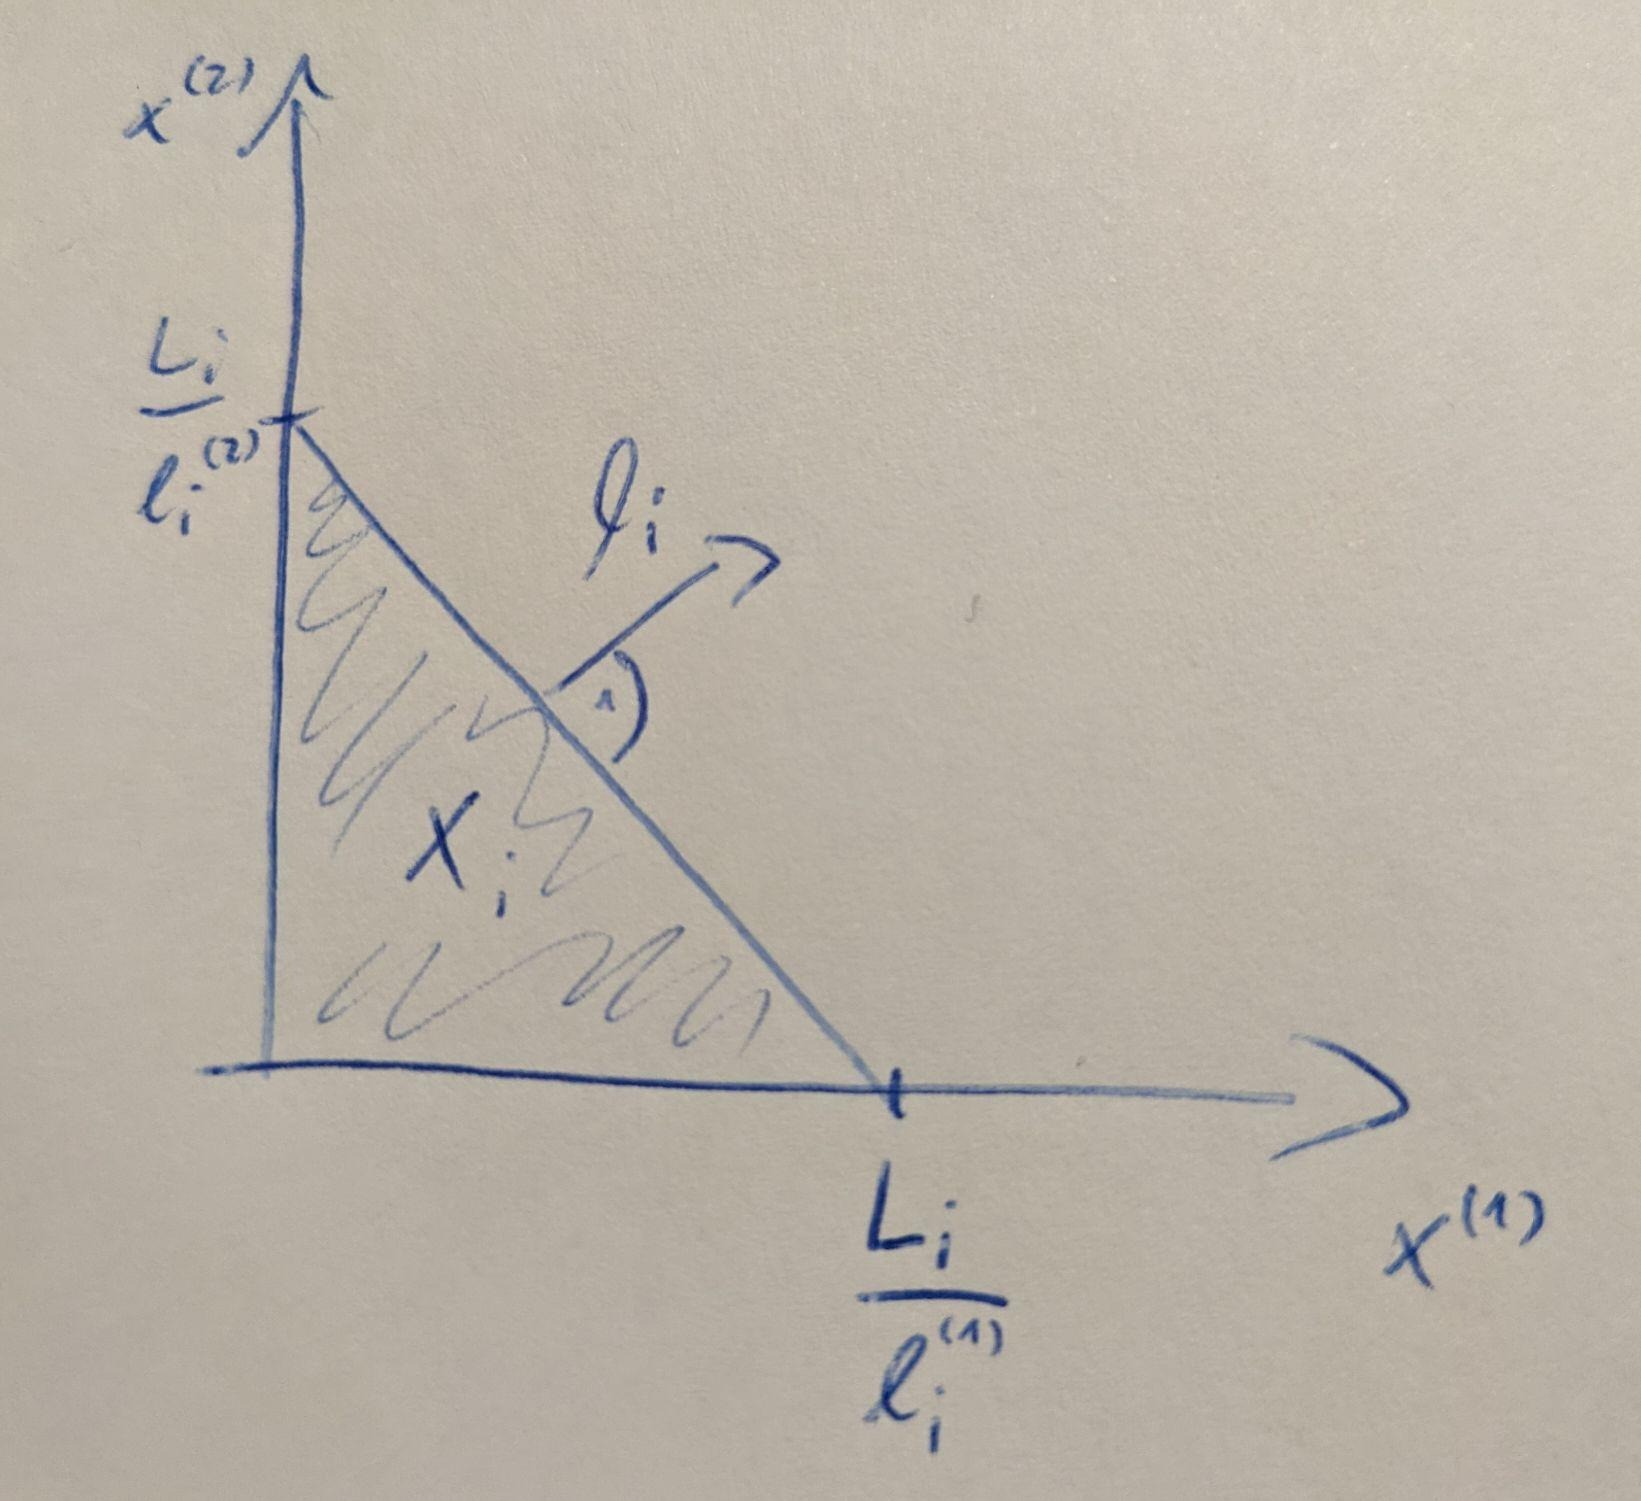
\includegraphics[width=0.46\textwidth]{images/pure-variable-cost.jpeg}
	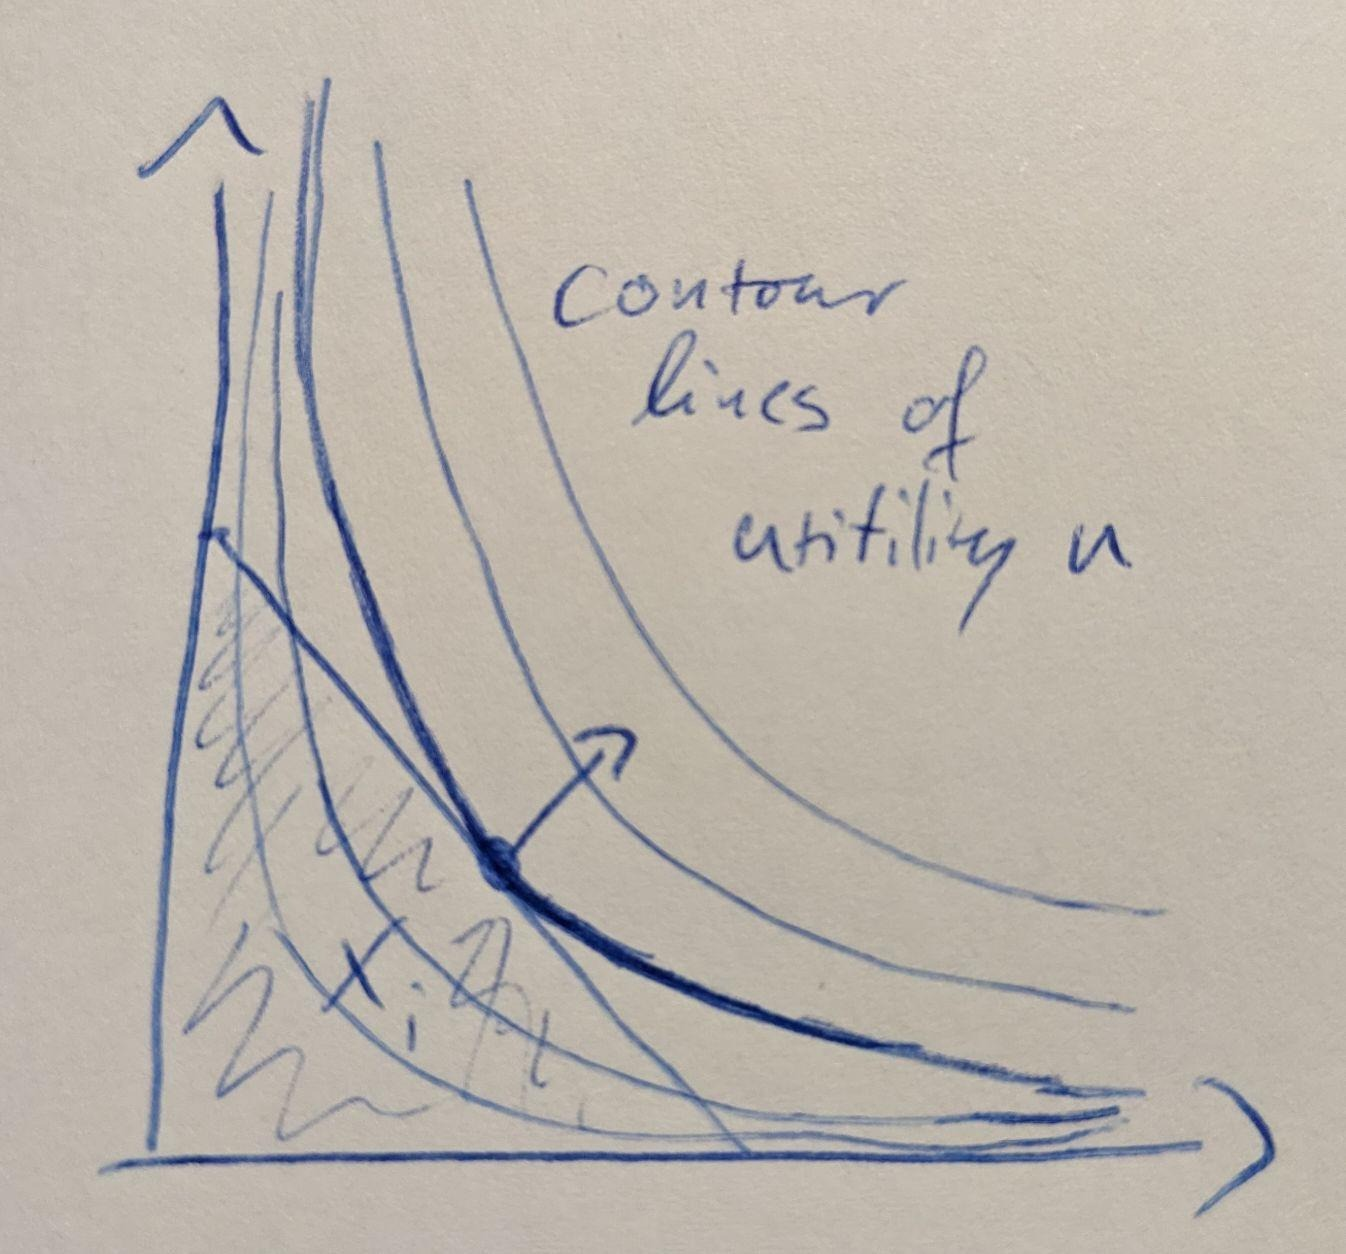
\includegraphics[width=0.45\textwidth]{images/hermit-decision-pure-variable.jpeg}
	\caption{
		Pure Variable Cost \(X_i\) on the left. The hermits decision problem
		on the right.
	}
\end{figure}
\begin{example*}[Pure Variable Costs]
	One important special case is
	\[
		X_i = \{ x \in \real_{\ge 0}^\dims: \langle x, l_i \rangle \le L_i \}.
	\]
	Here \(l_i^{(j)}\ge0\) is the labour time required by person \(i\) to produce one
	unit of good \(j\). Therefore the total time spent to produce quantity
	\(x^{(j)}\) of good \(j\) is \(x^{(j)}l_i^{(j)}\). Summing over all goods
	results in the total time requirement
	\[
		L_i(x) = \sum_{j=1}^\dims x^{(j)}l_i^{(j)} = \langle x, l_i\rangle,
	\]
	which obviously needs to be smaller than our time constraint \(L_i\).

	One could easily model exhaustion with \(L_i(x) = g(\langle x, l_i\rangle)\)
	for some strictly monotonously increasing function \(g\). You could also
	view \(L_i(x)\) more generally as the discomfort of labour instead of merely
	the time required, to generalize to tasks which take longer but are more
	enjoyable and vice versa.
\end{example*}

A hermit therefore faces the utility function maximization problem
\[
	\max_{L_i, x} u(\overbrace{1-L_i}^{\text{free time}}, x)
	\quad\text{subject to}\quad x\in X_i(L_i).
\]
going back to our special case, this has a very intuitive interpretation.


\begin{example*}[Pure Variable Costs]
	In the pure variable cost case, the hermits decision problem simplifies to
	\[
		\max_{x} u(\overbrace{1-L_i(x)}^{\text{free time}}, x).
	\]
	So denoting the partial derivative\footnote{
		If \(x\) was discrete one could replace derivatives with finite
		differences.  With concavity assumptions on \(u\), one could also make
		generalizations on the derivative (cf. subderivative) in the continuous
		case.
	}
	with regard to free time as \(u_f\) and
	the gradient vector with regard to \(x\) as \(u_x\), the first order
	condition for maximization requires
	\[
		0\overset!=\frac{du}{dx}
		= u_x - \nabla L_i(x) u_f
		= u_f \Bigl[
			\underbrace{\frac{u_x}{u_f}}_{\mathclap{\text{willingness to work (wtw)}}}
		- \overbrace{\nabla L_i(x)}^{\mathclap{\text{natural prices}}}
		\Bigr],
	\]
	where we can assume the marginal utility of more free time \(u_f\) to be
	positive. The natural prices are simply {\color{lightgray} a multiple of}
	\(l_i\)
	\[
		\nabla L_i(x) = {\color{lightgray} g'(\langle x, l_i\rangle) }l_i.
	\]
	In other words: the price of good \(j\), is the {\color{lightgray} marginal}
	time required to produce \(j\). And without exhaustion this is simply
	\(l^{(j)}_i\). If the willingness to work for good \(j\) is smaller than
	its price, then our gradient is negative in this direction. Meaning that
	a reduction of \(x^{(j)}\) would increase our utility. If \(\text{wtw}^{(j)}\) is
	greater than the price of \(j\), an increase of \(x^{(j)}\) increases utility.
\end{example*}
